\graphicspath{{../04ClassicalPhysics/pics/}}

\chapter{Classical Physics}\label{ch:ClassicalPhysics}
\lettrine[lines=2]{\color{darkocre}T}{he} concept of
\emph{operators}\index{Operator} extends the idea of functions. An unary numeric
function $f$ takes some numeric value $x$ as an input  and produces
another numeric value $y$:
\[
f\,x=y\quad \textrm{ or } \quad x\overset{f}{\longrightarrow} y\,.
\]
In mathematical jargon, $f$ \emph{maps} $x$ into $y$.

\begin{figure}[htbp]
  \centering
  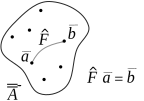
\includegraphics[scale=1.0]{arrowsOperatorGeneral}
  \caption{Operators extend the idea of functions. (a) An unary
    function $f$ can be applied to a number $x$ to produce
    another number $y$. (b) An unary operator $\op{F}$ can be applied to a vector
    $\vec{a}$ to yield another vector $\vec{b}$.}
  \label{fig:arrowsOperatorGeneral}
\end{figure}

\section{System}\label{sec:System}
An action of an operator $F$ on arrows can be represented symbolically
as an equation:
\[
F\,\vec{a}=\vec{b}\:.
\]
Often a ``hat'' is placed on top of an operator\footnote{In Quantum
Mechanics, for example.}, to emphasize that it is different from
numeric function:
\[
\colorboxed{red}{
  \op{F}\,\vec{a}=\vec{b}\:.
}
\]

\begin{mybio}{Simple Operators}\\
It is easy to come up with examples of operators:

\begin{itemize}
\item\phantom{x}

\item Unit operator (or \emph{identity} operator), such that
  \[
  \op{I}\,\vec{a}=\vec{a}\,.
  \]

\item ``Zeroing'' operator that maps every vector into a zero
  vector:
  \[
  \op{0}\, \vec{a} = \vec{0}\,.
  \]

\end{itemize}
\end{mybio}


To fully describe an operator, we must describe how it acts \emph{on
every} arrow. 

\begin{flushleft}
  {\bf Examples}
\end{flushleft}
Let us take a closer look at a couple of operators. While studying
these examples we must keep in mind that the relations between
components are \emph{specific to basis} and will change if we change the
basis. The question of how exactly the relation between components
changes will be addressed later in Section
\ref{sec:ComponentTransformation} for the simplest types of operators.


\begin{mybio}{Matrix}
Here is an example of matrix:
\[
\op{S} =
\begin{pmatrix}
  S_{11} & S_{12}\\
  S_{21} & S_{22}
\end{pmatrix} =
\begin{pmatrix}
  \alpha & 0\\
  0 & \alpha
\end{pmatrix}\,.
\]
Similar approach can be used to find the components of any linear operator.
\end{mybio}


\section{Oscillator}\label{sec:Oscillator}
An action of an operator $F$ on arrows can be represented symbolically
as an equation.

\section{State}\label{sec:State}
An action of an operator $F$ on arrows can be represented symbolically
as an equation.

\section{Dynamics}\label{sec:Dynamics}
An action of an operator $F$ on arrows can be represented symbolically
as an equation.

\section{Hamiltonian}\label{sec:Hamiltonian}
An action of an operator $F$ on arrows can be represented symbolically
as an equation.

\section{Lagrangian}\label{sec:Lagrangian}
An action of an operator $F$ on arrows can be represented symbolically
as an equation.

\section{Field}\label{sec:Field}
An action of an operator $F$ on arrows can be represented symbolically
as an equation.

\section{Ideal Versus Real}\label{sec:IdealVsReal}
An action of an operator $F$ on arrows can be represented symbolically
as an equation.



\section*{Chapter Highlights}
{\setstretch{1.5}\chhc
  \it  
\begin{itemize}
\item Operators extends the idea of functions.
\item Numeric functions (e.g., $\sin\,x$) act on numbers and yield
  other numbers. Operators may act on vectors to yield other vectors
  or numbers.
\item Linear operators represent the simplest and yet powerful class
  of operators on vectors.
\item Linear operators can be represented graphically or symbolically.
\end{itemize}

}
